\section{Background}

\subsection{Analysis of Orientation}

	Analyses of the simulated systems were performed to characterize the orientation of \suldiox in various environments above, within, and below the surface water region. The orientation of the surface molecules as \suldiox adsorbs and interacts with water is a property of any hydrate complex formation that takes places. Better understanding of the molecular orientational distributions will help elucidate the chemistry occurring during the adsorption process.

	The two molecules studied, \wat~and \suldiox, and similarly shaped with a C2$_v$ axis along their bisectors, and a molecular plane is defined by their three atoms. The orientational analyses presented herein focus on two angles used to define the molecular orientation in space. In each analysis a reference axis is used to define molecular angles, and is the z-axis unless otherwise specified. A ``tilt'' angle, $\theta$, defines the angle formed between a vector (generally the bisector vector pointing from the central atom in the direction of the other two atoms) and the positive reference axis. Thus the value of $\theta$ falls within a range of $[0,\pi]$. A second angle, $\phi$, defines the molecular ``twist'' around the reference axis. $\phi$ is formed between the projection of a vector onto the x-y reference plane, and the x-axis. $\phi$ is thus defined relative to the x-axis, and its values are in the interval $[-\pi,\pi]$. However, because of the symmetry of the \wat~and \suldiox~molecules and the equivalence of the two H or O atoms (in the \wat~or\suldiox, respectively), $\phi=-\pi$ is equivalent to $\phi=\pi$, and both situations are equivalent to $\phi=0$. Because $\phi=-\phi$, the value is reported within the range of $[0,\frac \pi 2]$. Figure \ref{fig:spherical-angle} shows the angle definitions using the z-axis as the reference axis.

\begin{figure}[h!]
	\begin{center}
		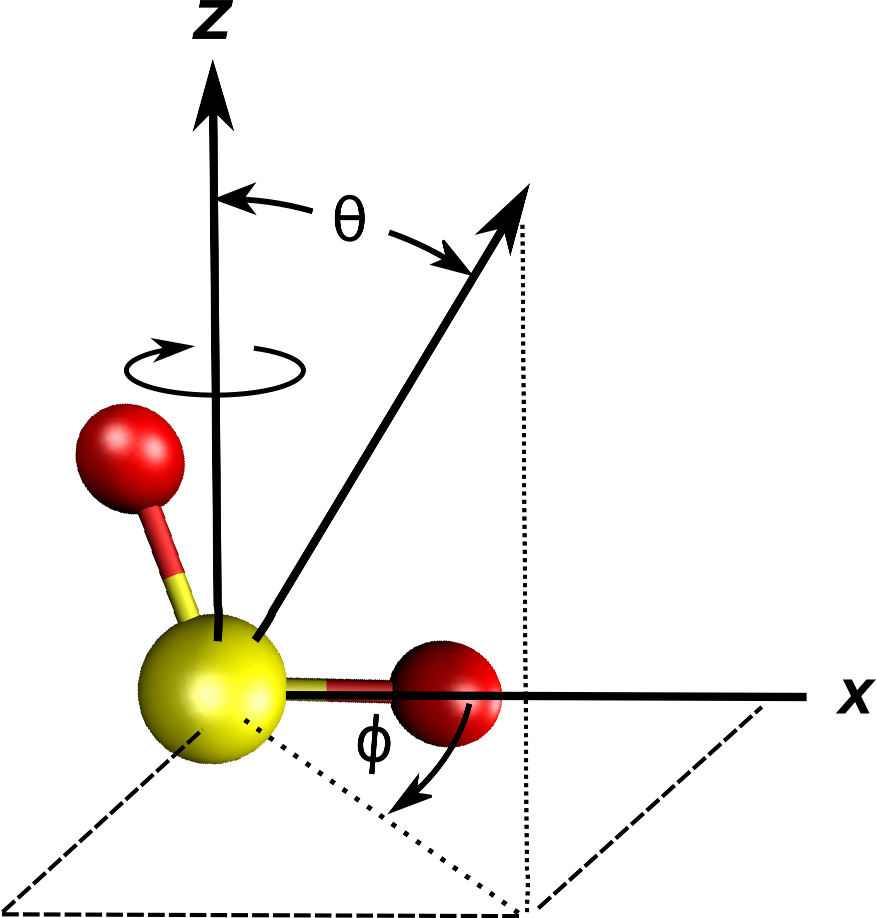
\includegraphics[scale=1.0]{images/sphericalanglegraphic.png}
		\caption{The visual representation of the angles $\theta$ and $\phi$ used to define molecular orientation of \suldiox~and \wat~relative to the reference axis. $\theta$ is the value of the ``tilt'' of the molecular bisector, and $\phi$ is the ``twist'' of the vector about the reference axis, starting at the x-axis.}
		\label{fig:spherical-angle}
	\end{center}
\end{figure}


\subsubsection{Water Orientation}
The orientation of water molecules at the 
\subsubsection{\suldiox~Orientation}

\subsection{Bonding Analysis}
\subsubsection{Nearest Neighbor}
\subsubsection{Hydrate Complex Formation}
